\documentclass{report}
\usepackage{preamble}

\begin{document}

\begin{titlepage}
  %\vspace*{\fill}
  \begin{minipage}{0.4\textwidth}
    \begin{flushleft} \large
      \hspace*{-0.5cm}
      
\includegraphics[scale=0.4]{eng-uoi-logo}\\
    \end{flushleft}
  \end{minipage}\\
  \center
  \textsc{\LARGE University of Ioannina\\[0.1cm] School of Engineering}\\[0.5cm]
  \textsc{\Large Department of Computer Science and Engineering}\\[0.4cm]
  \textsc{\Large Diploma Thesis}\\[1cm]

  \LARGE \textbf{Enabling NIPoPoW Applications on Bitcoin Cash} \\[1cm] 

  \begin{minipage}{0.4\textwidth}
    \begin{flushleft} \large
      \emph{Author:} \\
      Kostis \textsc{Karantias}\\
      ID: \emph{2454}
    \end{flushleft}
  \end{minipage}
    ~
  \begin{minipage}{0.5\textwidth}
    \begin{flushright} \large
      \emph{Supervisor:} \\
      Prof. Leonidas \textsc{Palios}
    \end{flushright}
  \end{minipage}\\[1cm]

  {\large February 2019}
  %\vspace*{\fill}
\end{titlepage}

\newpage

\thispagestyle{empty}
\null

\newpage

More detailed title page.
\thispagestyle{empty}

\newpage

\thispagestyle{empty}
\null

\newpage

\begin{abstract}
  In this work we examine the real-world applications of the recent blockchain primitive called Non Interactive Proofs of Proof of Work (NIPoPoWs). We enable the use of the primitive on Bitcoin Cash by implementing the first known velvet fork on a blockchain. We provide concrete implementations for creating a velvet fork, and generating proofs on a blockchain that has been forked in this way.
\end{abstract}

\newpage

\tableofcontents

\newpage

\chapter{Introduction}

\section{Motivation}
\emph{Cryptocurrencies} are digital assets that utilize cryptography in order to allow value transfer, without the need of a central party or trusted authority. The technology originally appeared in 2008 in a paper by Satoshi Nakamoto~\cite{bitcoin} as Bitcoin, along with a reference implementation in C++. It didn't take long until a community of enthusiasts and cryptographers embraced the technology and started studying it and using it extensively. New cryptocurrencies based on Bitcoin's ideas and codebase started popping up, among them most notably Litecoin and Dogecoin.

This work clearly was a huge inspiration. In 2014 Ethereum~\cite{ethereum} appeared, which aimed to do much more than just value transfers: it built on Nakamoto's ideas in order to build a world computer. Programs called \emph{smart contracts} could be stored and run on a decentralized manner. Such smart contracts gave us the ability to write immutable contracts, where \emph{code is law}.

Few years later and the landscape is completely changed. More and more cryptocurrencies are created every single day. Public interest and prices have skyrocketed. There is lots of optimism about the future decentralized techologies such as Bitcoin can bring, mainly a democratization of money, usually called "banking the unbanked".

However, being more widespread and popular surfaced some problems the most important of which is scalability. Technically, each cryptocurrency has a \emph{blockchain}, which is literally a chain of \emph{blocks} linked together like a linked list. These blocks contain \emph{transactions}. Every transaction needs to be recorded and stored in a block, and everyone has to know about it. As a result, the Bitcoin blockchain is 185GB at the time of writing. The Ethereum blockchain comes at 667GB. Typically, for someone to participate on the network, and do actions like send transactions they have to download the whole blockchain. However at such rates it is very time-consuming and resource-intensive or even impossible for someone to download a chain. So called \emph{lite nodes} that don't need to download the whole chain do exist, but at best they need information linear to the size of the chain, so they're a constant-factor improvement.

New cryptocurrencies with interesting features pop up all the time. There's long been an interest in implementing sidechains~\cite{sidechains}, as a way to interoperate between two blockchains. One should be able to trustlessly transfer his Bitcoin to another chain and use it there, and transfer it back if he so desires. TODO

\section{Related Work}
\section{Objectives}
\section{Structure}

\chapter{Background}
\section{Primitives}
\subsection{Cryptographic Hash Functions}
A \textit{hash function} is a function used to map data of arbitrary size to data of a fixed size. Formally, a hash function $H$ is of the form $H: D \rightarrow [0, 2^\kappa)$, where $\kappa$ is a characteristic of $H$, specifically the number of bits of its output.

For a hash function to be a cryptographic hash function it has to satisfy the following properties:
\begin{itemize}
  \item \textbf{Pre-image resistance}: Given a hash of $h$ it should be difficult to compute an input $m$ such that $H(m) = h$.
  \item \textbf{Second pre-image resistance}: Given an input $m_1$ it should be difficult to compute an input $m_2$ such that $H(m_1) = H(m_2)$.
  \item \textbf{Collision resistance}: It should be difficult to compute two inputs $m_1$ and $m_2$ such that $H(m_1) = H(m_2)$.
\end{itemize}

Bitcoin utilizes two hash functions, SHA256 ($\kappa=256$) and RIPEMD160 ($\kappa=160$).

This work and the works it is based on \cite{nipopows} operate under the Random Oracle model where hash functions are assumed to have uniformly distributed outputs in their output domain, meaning that $\forall x, y: Pr[H(x) = y] = \frac{1}{2^\kappa}$.

\subsection{Public-key Cryptography}
Each user is assumed to have a \textit{key pair} composed of a \textit{public key} which can be shared freely and a \textit{private key} which should be kept secret. A public-key cryptographic system should implement the following operations:

\begin{itemize}
  \item $Encrypt_{public}(m)$
  \item $Decrypt_{private}(m)$ where $\forall m: \exists! enc: Decrypt_{private}(enc) = m \land enc = Encrypt_{public}(m)$ and it is difficult for someone without $public$ to create such an $enc$
  \item $Sign_{private}(m) = Encrypt_{private}(m)$
  \item $Verify_{public}(m) = Decrypt_{public}(m)$ where $\forall m: \exists! sig: Verify_{public}(sig) = True \land sig = Sign_{private}(m)$ and it is difficult for someone without $private$ to create such a $sig$
\end{itemize}

Bitcoin utilizes \textit{ECDSA}, which is based on elliptic curves, as its public-key cryptography implementation.

\subsection{\label{sec:merkle-trees}Merkle Trees}
A Merkle tree~\cite{merkle} is a data structure which allows a party to commit to a set of items using only a single hash, and prove the inclusion of any item in the committed set by providing a logarithmic proof in terms of the cardinality of the set.

More specifically, the hashes of the items consist the leafs of the tree, and the last level. The internal levels are defined recursively as follows: To create level $k-1$ each pair of level $k$ $(A, B)$ is transformed as a node of value $H(A || B)$ which points to both $A$ and $B$. If the number of nodes at level $k$ is odd, the last node at that level is paired with itself.
\footnote{This specific construction is the one Bitcoin implements. There are various other constructions which are not inside the scope of this paper.}

Merkle trees are useful in Bitcoin in order to commit to a set of transactions to be included in a block while keeping the block header of a constant size as we will see shortly.

To provide proof of inclusion, all a prover has to do is provide a path of siblings up to the root $\sf{siblings}$ and a bit vector $\sf{left}$ indicating whether each sibling is on the left or the right. The verification process is shown in Algorithm~\ref{alg:merkle-verification}.

\begin{algorithm}[H]
  \caption{\label{alg:merkle-verification}The \textsf{Verify} algorithm
    for a Merkle proof}
    \begin{algorithmic}[1]
      \Function{\sf Verify$_{\sf root}$}{\sf leaf, siblings, left}
            \Let{\sf{currentHash}}{\sf{leaf}}
            \While{$\sf{left} \neq []$}
              \Let{\sf{siblingIsLeft}}{\sf{left.shift()}}
              \If{\sf{siblingIsLeft}}
                \Let{\sf{currentHash}}{H(siblings.shift() || currentHash)}
              \Else
                \Let{\sf{currentHash}}{H(currentHash || siblings.shift())}
              \EndIf
            \EndWhile
            \State\Return{currentHash = root}
        \EndFunction
    \end{algorithmic}
\end{algorithm}

An example of a Bitcoin Merkle tree, along with a proof of inclusion for $K$ can be seen on Figure~\ref{fig:merkletree}.

\begin{figure}
  \centering
  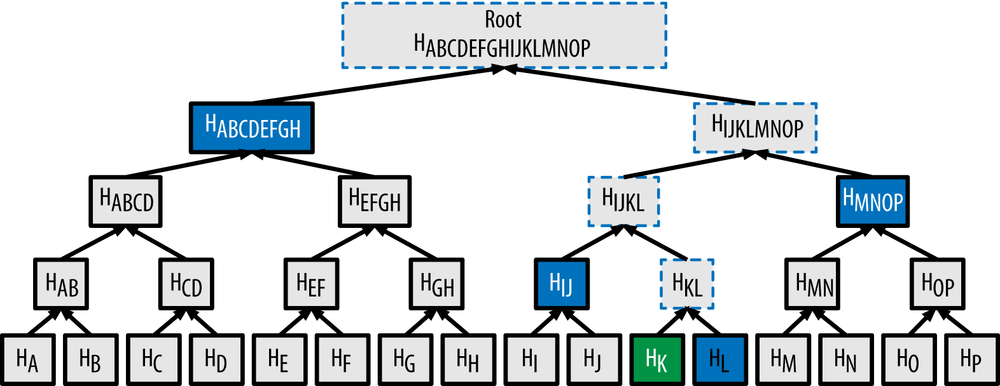
\includegraphics[width=0.9\columnwidth,keepaspectratio]{figures/merkle-tree-proof.png}
  \caption{A Bitcoin Merkle tree. Source:~\cite{mastering}}
  \label{fig:merkletree}
\end{figure}

\subsection{Bloom Filters}

\section{Bitcoin}
Bitcoin was introduced in 2008 by Satoshi Nakamoto~\cite{bitcoin} as a
peer-to-peer version of electronic cash, allowing online payments to be sent
directly between parties without the need of a intermediary.

Transfer of value in Bitcoin happens with transactions. A transaction has
inputs and outputs. An output is where the value creation happens for the
receiver. An output can be later redeemed by using its designated receiver's
private key and turned into an input to be used for another transaction.

TODO

\subsection{Block Structure}
A block header contains mainly the hash of the previous block, a Merkle root
hash to commit to a set of transactions, and a nonce.

After the block header comes the series of transactions included in the block.

TODO

\subsection{Proof of Work}
\subsection{Merkle Trees}
A Merkle tree~\cite{merkle} is a data structure which allows a party to
commit to a set of items using only a single hash, and prove the inclusion of
any item in the committed set by providing a logarithmic proof in terms of the
cardinality of the set.

More specifically, the hashes of the items consist the leafs of the tree, and
the last level. The internal levels are defined recursively as follows: To
create level $k-1$ each pair of level $k$ $(A, B)$ is transformed as a node
of value $H(A || B)$ which points to both $A$ and $B$. If the number of nodes
at level $k$ is odd, the last node at that level is paired with itself.
\footnote{This specific construction is the one Bitcoin implements. There are
various other constructions which are not inside the scope of this paper.}

Merkle trees are useful in Bitcoin in order to commit to a set of
transactions to be included in a block while keeping the block header of a
constant size.

To provide proof of inclusion, all a prover has to do is provide a path of
siblings up to the root $\sf{siblings}$ and a bit vector $\sf{left}$ indicating
whether each sibling is on the left or the right. The verification process is
shown in Algorithm~\ref{alg:merkle-verification}.

\begin{algorithm}[H]
  \caption{\label{alg:merkle-verification}The \textsf{Verify} algorithm
    for a Merkle proof}
    \begin{algorithmic}[1]
      \Function{\sf Verify$_{\sf root}$}{\sf leaf, siblings, left}
            \Let{\sf{currentHash}}{\sf{leaf}}
            \While{$\sf{left} \neq []$}
              \Let{\sf{siblingIsLeft}}{\sf{left.shift()}}
              \If{\sf{siblingIsLeft}}
                \Let{\sf{currentHash}}{H(siblings.shift() || currentHash)}
              \Else
                \Let{\sf{currentHash}}{H(currentHash || siblings.shift())}
              \EndIf
            \EndWhile
            \State\Return{currentHash = root}
        \EndFunction
    \end{algorithmic}
\end{algorithm}

An example of a Bitcoin Merkle tree, along with a proof of inclusion for $K$ can be seen on Figure~\ref{fig:merkletree}.

\begin{figure}
  \centering
  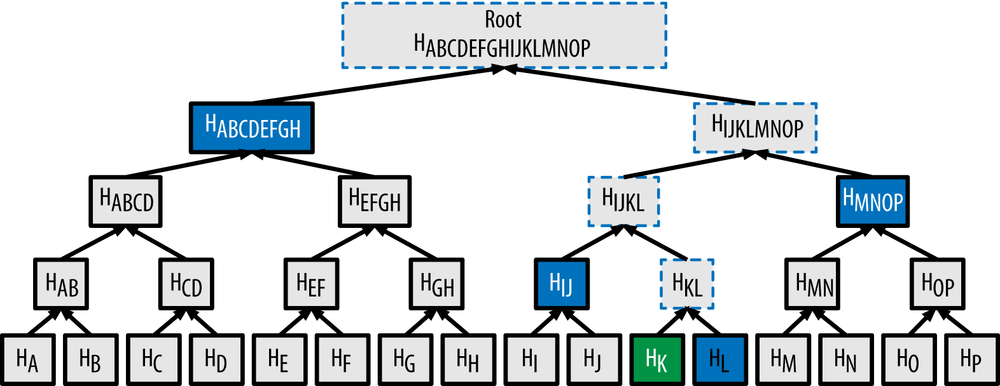
\includegraphics[width=0.9\columnwidth,keepaspectratio]{figures/merkle-tree-proof.png}
  \caption{A Bitcoin Merkle tree. Source:~\cite{mastering}}
  \label{fig:merkletree}
\end{figure}

\subsection{Simplified Payment Verification}
The size of the blockchain has reached 185GB by September 2018, which makes
it a very time consuming or even infeasible process to synchronise a full
node. Fortunately, a solution was proposed in the original whitepaper
~\cite{bitcoin}, which allows the creation of so-called \textit{lite nodes}.
Lite nodes only know the headers of the entire blockchain, which are
constant-size for each block (80 bytes). At the time of writing of this
paper, the size of all block headers was $\sim$42MB. The lite node then asks the
network for transactions concerning it (e.g.\ transactions concerning a
specific public key). Full nodes of the network find such transactions and
return them to the requester. For each transaction, the block header of the
block it's included in is returned, along with a Merkle tree proof of
inclusion which the lite node can then verify. This protocol is reliable as
long as an adversary does not control the network of a lite node.

\subsection{Bitcoin Cash}
In 2017 Bitcoin faced severe scalability issues~\cite{onscaling}. Its limited
1MB block size meant that it could only support a maximum of 7 transactions per
second. As Bitcoin's popularity had exploded at the time, the problem was
hugely exacerbated. The most prominently proposed solution for this was a block
size increase, however no consensus was reached. The discussions ended with a
fork of the main Bitcoin chain which allowed for 8MB blocks, called Bitcoin
Cash.

\section{Non-Interactive Proofs of Proofs of Work}
Seeing that proofs are linear in the chain length, it is natural to consider if we can do better. NIPoPoW \cite{nipopows} provides the first family of succinct proofs which are logarithmic in the size of the chain and proven secure in the Backbone \cite{backbone} protocol.

There have been previous attempts to create proofs smaller in size than SPV proofs~\cite{KLS}, where a scheme for logarithmic proofs was proposed.  This scheme was later proven insecure~\cite{nipopows}.

\subsection{Terminology}
NIPoPoWs are categorized in two kinds of proofs:

\begin{itemize}
  \item We have a valid chain where the last $k$ blocks (also called the \textit{unstable} part of the chain) are the ones we're claiming. This is called a \textbf{suffix proof}.
  \item We have a valid chain where a specific given block is included in its \textit{stable} part (excluding the last $k$ blocks). This is called an \textbf{infix proof}.
\end{itemize}

\subsection{Assumptions}
An assumption NIPoPoWs make is that the difficulty is constant. This is not true for Bitcoin or Bitcoin Cash.

% further analysis in |
%                     \/
% cite variable difficulty backbone TODO

NIPoPoWs also assume each block contains an interlink data structure, which we'll study shortly. Interlinks too don't exist in Bitcoin or Bitcoin Cash.

In the next section we'll look at how we sidestep all those issues.

\subsection{Levels}
At the heart of the primitive lies the separation of blocks into levels. The level of a block is defined as $\textit{level}(B) = \left \lfloor \log(T) - \log(\sf{id}(B)) \right \rfloor$, where $T$ is the constant difficulty of the blockchain. The genesis block is an exception to this rule as $\textit{level}(Gen) = \infty$. We call a block of level $\mu$ a $\mu$-superblock.

Intuitively, the level of a block is the number of leading zeros of the binary representation of the block id when left padded to the length of $T$. An example of this can be seen on Table~\ref{table:level-counting}.

\begin{table}
  \centering
  \begin{tabular}{|c|c|}
    \hline
    $T$ & 1110000 \\
    \hline
    $\sf{id}(B)$ & \underline{000}1000 \\
    \hline
  \end{tabular}
  \caption{Calculating the level of a block by counting the leading zeros (3 in this case).}
  \label{table:level-counting}
\end{table}

Figure~\ref{fig:hierarchy} shows an example the implied blockchain created from the superblocks.

\begin{figure}
  \centering
  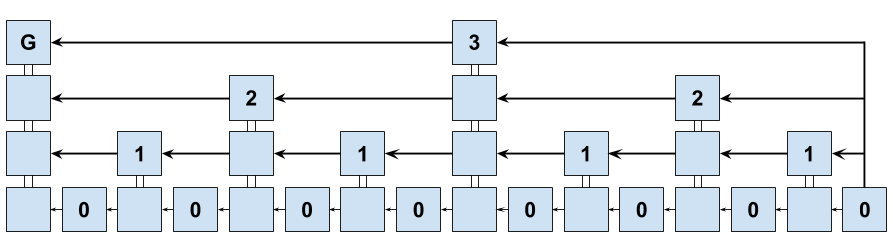
\includegraphics[width=0.9\columnwidth,keepaspectratio]{figures/hierarchical-ledger.png}
  \caption{The hierarchical blockchain.  Higher levels have achieved a lower target (higher difficulty) during mining. All blocks are connected to the genesis block $G$. Source:~\cite{nipopows}}
  \label{fig:hierarchy}
\end{figure}

\subsection{Notation}
The NIPoPoWs paper introduces some notation for talking about blockchains with levels which we'll be using extensively. The notation is widely influenced by Python. Specifically:

\begin{itemize}
  \item $\chain$ denotes a blockchain, with $\chain[0]$ being the genesis block, $\chain[k]$ being the $k$-th first block and $\chain[-k]$ being the $k$-th last block.
  \item $\chain[k:]$ denotes the sub-blockchain starting from the $k$-th block, $\chain[-k:]$ denotes the sub-blockchain starting from the $k$-th last block.
  \item $\chain[:k]$ denotes the sub-blockchain ending before the $k$-th block, $\chain[:-k]$ denotes the sub-blockchain ending before the $k$-th last block.
  \item $\chain[i:j]$ denotes the sub-blockchain starting from the $i$-th block and ending at the $j$-th block. $i$ and $j$ can also be negative numbers similar to above.
  \item $\chain\{B:\}$ denotes the sub-blockchain starting from the block with block id $B$.
  \item $\chain\upchain^\mu$ denotes the sub-blockchain of $\chain$ where all blocks are of level $\mu$ or higher.
\end{itemize}

\subsection{Interlink}
Instead of keeping only the hash of the previous block inside the block header, for every superblock level we keep a pointer to the most recent superblock of that level. The structure containing these pointers is called the interlink. Bitcoin does not support such a structure in the block header but we will study how to sidestep this issue by velvet forking in a few sections.

\begin{table}
  \centering
  \begin{tabular}{|c|c|}
    \hline
    Level & Block \\
    \hline
    $0$ & $C[-2]$ \\
    $1$ & $C[-2]$ \\
    $2$ & $C[-4]$ \\
    $3$ & $C[-8]$ \\
    $\infty$ & $C[0]$ \\
    \hline
  \end{tabular}
  \caption{Interlink of $C[-1]$ from Figure~\ref{fig:hierarchy}}
  \label{table:interlink-example}
\end{table}

It's important to note that the interlink can be encoded as a series of block ids, starting from $0$ up to $\infty$. It can also be compressed by using this series as the leafs of a Merkle tree and taking the Merkle tree root.

Suppose we have a block $B'$ with an interlink stored as $B'.{\sf interlink}$. In order to produce the interlink for a block after $B'$ we make sure to change all pointers from level $0$ up to $level(B')$ to point to $B'$, as $B'$ will be the most recent block at these levels (remember that a block of level $\mu$ is also of level $\mu-1$). We call this procedure {\sf updateInterlink}, which can be seen in detail on Algorithm~\ref{alg.nipopow-interlink}.

\begin{algorithm}[H]
    \caption{\label{alg.nipopow-interlink}updateInterlink}
    \begin{algorithmic}[1]
        \Function{\sf updateInterlink}{$B'$}
            \Let{\textsf{interlink}}{B'.\textsf{interlink}}
            \For{$\mu = 0$ to $\textit{level}(B')$}
                \Let{\textsf{interlink}[\mu]}{\textsf{id}(B')}
            \EndFor
            \State\Return{\textsf{interlink}}
        \EndFunction
    \vskip8pt
    \end{algorithmic}
\end{algorithm}


\subsection{Suffix Proofs}
Suffix proofs are parameterized by $k$ and $m$. $k$ refers to the number of blocks that need to bury a block for it to be considered stable.

A suffix proof of a chain $\chain$ is constituted of two chains, $\pi$ and $\chi$. The final proof is the concatenation of those two chains $\pi \chi$. $\chi$ always refers to the chain of unstable blocks and is evaluated as $\chi = \chain[-k:]$.

The process for constructing $\pi$ is a little more convoluted. First we have to find the first level $\mu$ where $|\chain\upchain^\mu| \ge m$. We call this level $max\mu$. For this level we take all its blocks except for the last $m$: $\pi_{max\mu} = \chain\upchain^\mu[:-m]$. Then for every level $\mu$ from $max\mu - 1$ to $0$, we take blocks $\pi_\mu = \chain\upchain^\mu [:-m]\{\chain\upchain^{\mu+1}[-m]:\}$.

$\pi$ is then evaluated as the concatenation of all those chains starting from the oldest block:

$$ \pi = \pi_{max\mu} || \pi_{max\mu-1} || \ldots || \pi_0 $$

\begin{figure}
  \centering
  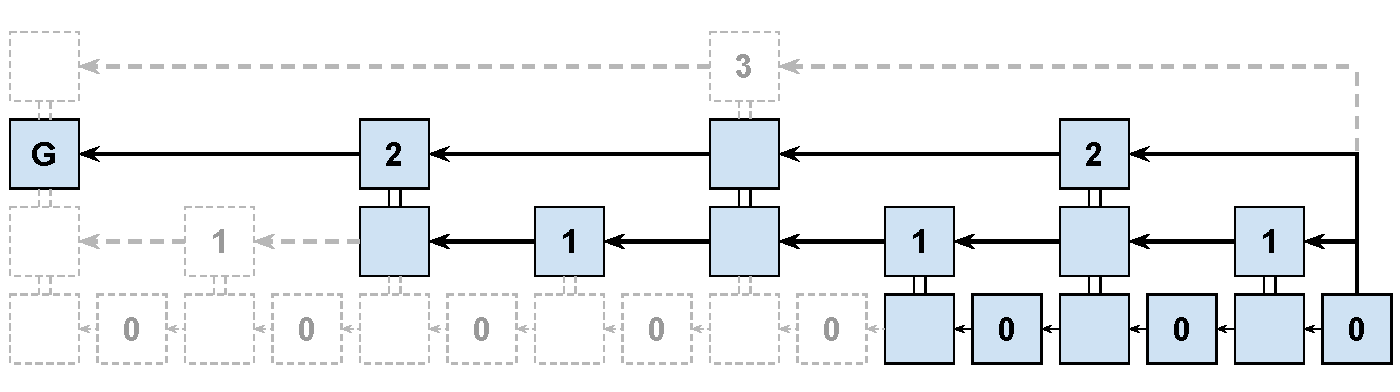
\includegraphics[width=0.9\columnwidth,keepaspectratio]{figures/non-interactive-popow.pdf}
  \caption{Construction of $\pi$ of a suffix proof. $m=3$  Source:~\cite{nipopows}}
  \label{fig:suffix-proof}
\end{figure}

It's important to notice that the chain provided to the verifier is an actual chain: one can start at the end and traverse it until the genesis block by utilizing the interlink of each block, similar to how they would do that on a conventional blockchain by using each block's $\sf previd$.

\subsection{Infix Proofs}
\label{ssec:infix}
For the verifier to be able to determine a predicate on one or more blocks ($\chain' \subseteq \chain$) of our chain, we have to make sure we include them in a proof. A suffix proof is not guaranteed to include all blocks of interest in $\chain'$. In order to include these we have to make sure they are linked to the proof, e.g. that the proof chain is a traversable. To this end, let's assume some arbitrary block $B \in \chain'$. Let's also assume an existing suffix proof $\pi\chi$. We find blocks $E'$ and $E$ on the suffix proof, such that:

\begin{itemize}
  \item $E$ is the next block after $E'$ on the proof
  \item $B$ comes before $E$ on $\chain$
  \item $B$ comes after $E'$ on $\chain$
\end{itemize}

An example of such a triplet of blocks satisfying those conditions can be seen on Figure~\ref{fig:infix-proof}.

\begin{figure}
  \centering
  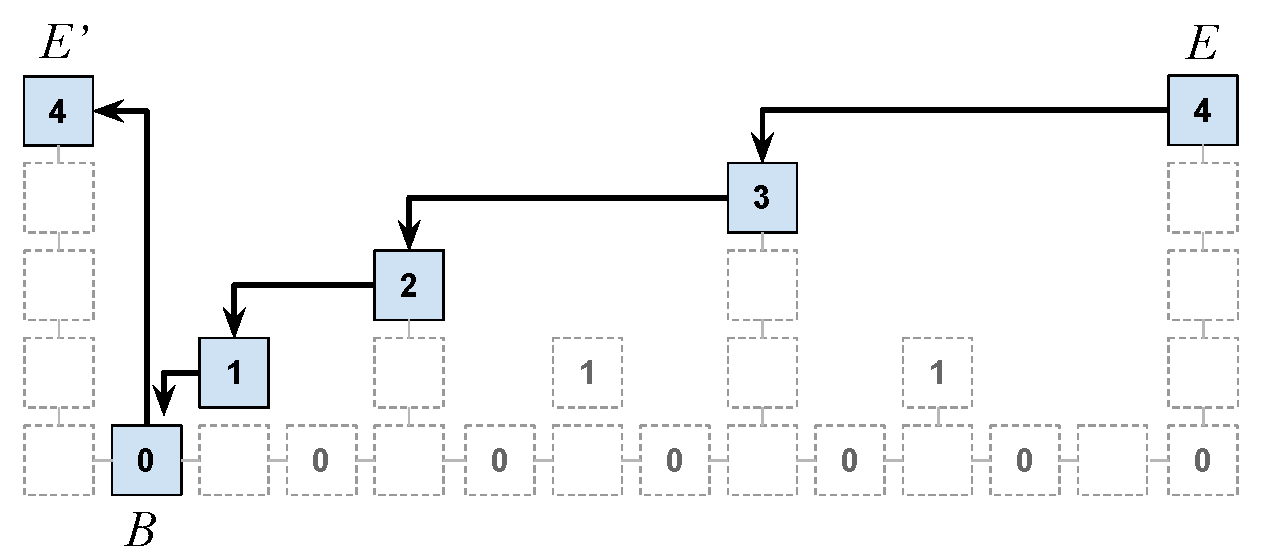
\includegraphics[width=0.9\columnwidth,keepaspectratio]{figures/infix.pdf}
  \caption{Construction of an infix proof.  Source:~\cite{nipopows}}
  \label{fig:infix-proof}
\end{figure}

We then perform a procedure called $\sf followDown$ in order to figure out which blocks need to be added to the proof in order to link $E$ to $B$. $\sf followDown$ includes blocks on intermediate levels until $B$ is reached. The full algorithm can be seen on Algorithm~\ref{alg.nipopow-infix-follow}.

\begin{algorithm}[H]
    \caption{\label{alg.nipopow-infix-follow}The \textsf{followDown} function
    which produces the necessary blocks to connect a superblock $E$ to a
    preceeding regular block $B$.  Source:~\cite{nipopows}}
    \begin{algorithmic}[1]
        \Function{\sf followDown}{$E$, $B$, \textsf{height}} %, realLink, blockById}
            \State{$aux \gets \emptyset$; $\mu \gets \textit{level}(E)$}
            \While{$E \neq B$}
                \Let{B'}{\textsf{blockById}[E\text{.interlink}[\mu]]}
                \If{$\textsf{height}[B'] < \textsf{height}[B]$}
                    \Let{\mu}{\mu - 1}
                \Else
                    \Let{aux}{aux \cup \{E\}}
                    \Let{E}{B'}
                \EndIf
            \EndWhile
            \State\Return{$aux$}
        \EndFunction
    \vskip8pt
    \end{algorithmic}
\end{algorithm}


Augmenting the original suffix proof with the new blocks provided by $\sf followDown$ on all our blocks of interest $B \in \chain'$ gives us our final infix proof. Note that as was the case with our suffix proofs, the infix proof is traversable.

% TODO: I never talk about the infix predicate

\subsection{Proof Verification}
% TODO

\subsection{Velvet Forks}
Velvet forks~\cite{nipopows,velvet} describe a formalization of adding arbitrary data inside blocks in order to allow potential applications without sacrificing the backwards compatibility of the blockchain.

Miners who are willing to contribute to the fork can add data of interest in the form of coinbase transaction data. 

Backwards compatibility is achieved by not changing the consensus rules, meaning that set of acceptable blocks does not change. So any block that was acceptable remains acceptable even if it does not contain any data concerning the fork, or if it contains invalid data.

\subsection{User-Activated Velvet Forks}
In case miners aren't interested in including such data, users can also create such a fork by making a kind of transaction called velvet transaction. In a velvet transaction a user includes any data of interest in unspendable transaction outputs (like OP\_RETURN).

For the consumer of such data, the only difference is that they have to look inside the whole block to find it, not only inside the coinbase data.

Such forks come at the cost of making such transactions, because the user who makes the fork needs to pay transaction fees every time they wish to add data to the blockchain.

For our application, we implemented a User-Activated Velvet Fork in order to add the interlink data structure to Bitcoin Cash blocks. Since Bitcoin Cash has very low fees, a projection of running such a fork comes at around 10€/month.


\chapter{Velvet Fork Implementation}
We implement ... motivation TODO ...

\pdffigure{blocks-with-their-interlinks}{Example of blocks with their corresponding interlinks for $T = 100000$. Note that for the upcoming block marked with \textbf{?} we can produce its interlink without knowing its hash.}

Since Bitcoin Cash blocks don't contain the interlink we have to utilize a User-Activated Velvet Fork. To this end, we need to make sure that a transaction is included in every single block containing its implied interlink. We do this by implementing a service which for every new block, calculates the expected interlink of the upcoming block and sends a transaction including this interlink in hopes that it will be included in the upcoming block. If this is indeed achieved then that block will indeed contain its valid interlink. We henceforth call the service which does this an \emph{interlinker}. An example of blocks and their corresponding interlinks can be seen on Figure~\ref{fig:blocks-with-their-interlinks}.

\section{Picking a Velvet Genesis}
Naturally one would expect the interlink to start from the real blockchain genesis as it would enable proofs for any already existing block of that blockchain. However, for older blocks there can be no improvement. There is no other option than providing the full chain as a proof since no older blocks contain any interlinks. Thus in order to avoid accounting in our interlink for blocks in the past that can only be connected to the real genesis by supplying the full chain we choose a new genesis called the \emph{velvet genesis}. For our purposes in Bitcoin Cash testnet we chose the block with height 1257603 as our velvet genesis.

\section{Interlink encoding}
We now have to consider our options for representing the interlink. 
Bitcoin Cash uses SHA-256 for the block hashes, meaning that each block id consists of 32 bytes. 
A naive encoding would be one where each 32-byte block hash from level $0$ up to $\infty$ is concatenated, with the $\infty$ pointer always pointing to the genesis block..
For 35 levels, which according to Figure~\ref{fig:bitcoin-cash-testnet-levels-after-velvet-genesis} is a reasonable figure, this encoding would take approximately 1.12KB.
Considering that \code{OP\_RETURN} scripts are limited in size to 223 bytes, this would only allow us to include up to 6 pointers at best.

\begin{figure}
  \centering
  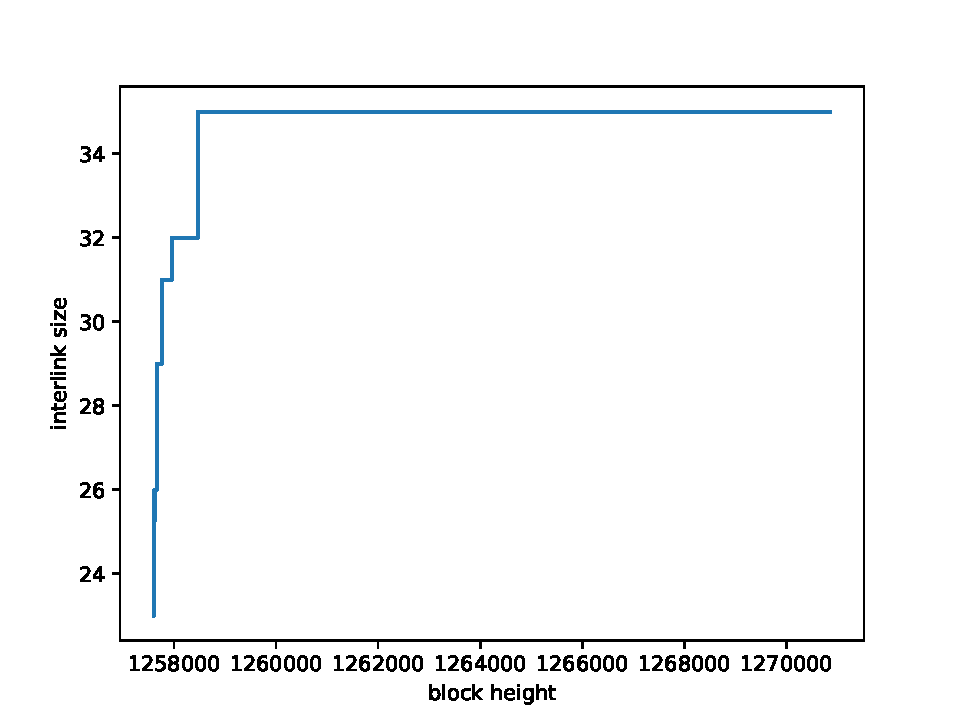
\includegraphics[width=0.9\columnwidth,keepaspectratio]{figures/bitcoin-cash-testnet-levels-after-velvet-genesis.pdf}
  \caption{Number of levels assuming our selected velvet genesis.}
  \label{fig:bitcoin-cash-testnet-levels-after-velvet-genesis}
\end{figure}

Putting this limitation aside, the fee of the transaction is proportional to the transaction size, and since we're going to be sending a transaction for every block (which is mined approximately every 10 minutes), it is important that the fee is minimized.

Thus in order to save space, we only include a commitment to the interlink in our transactions. Specifically, we take the Merkle Tree root of the Merkle Tree with leafs the block hashes starting from level $0$ up to $\infty$. This way, our interlink encoding is constant size and we can easily provide compact proofs for any of the levels.

\section{Discoverability}
We've talked about how just including the interlink somewhere on a block is what really matters but it is crucial that we make this information easy to discover. We achieve this in two ways. First, we include the interlink commitment inside a special \code{OP\_RETURN} output. Such outputs are already being used for storing arbitrary data in blocks~\cite{arbitrary-data} therefore we adopt this method for storing our interlinks. Second, we aim to make this interlink discoverable for lite nodes, so we don't require our users to download a whole block in order to look into it. We achieve this by utilizing a method called \emph{SPV tagged outputs}~\cite{spv-tagged}.

SPV tagged outputs are outputs that are tagged so that they can be discovered by SPV nodes who add the ``tag'' to the filter. Specifically, we form outputs of the form \code{OP\_RETURN baba deadbeef}, where \code{baba} is our tag and \code{deadbeef} is our payload (in our case, the interlink commitment). A bloom filter for \code{baba} will then match this output and subsequently the transaction that contains it and this is how our specialized SPV nodes can discover our outputs. The full nodes forwarding the velvet transactions to the SPV nodes don't have any knowledge of what a velvet fork even is, let alone that they are forwarding its transactions.

The tag we use for our transactions is \code{696e7465726c696e6b}, which is the ASCII encoding of \code{interlink}. An example of such a real-world velvet transaction created by our deployed interlinker on the Bitcoin Cash testnet can be seen on Figure~\ref{fig:actual-velvet-tx}.

\begin{figure}
  \centering
  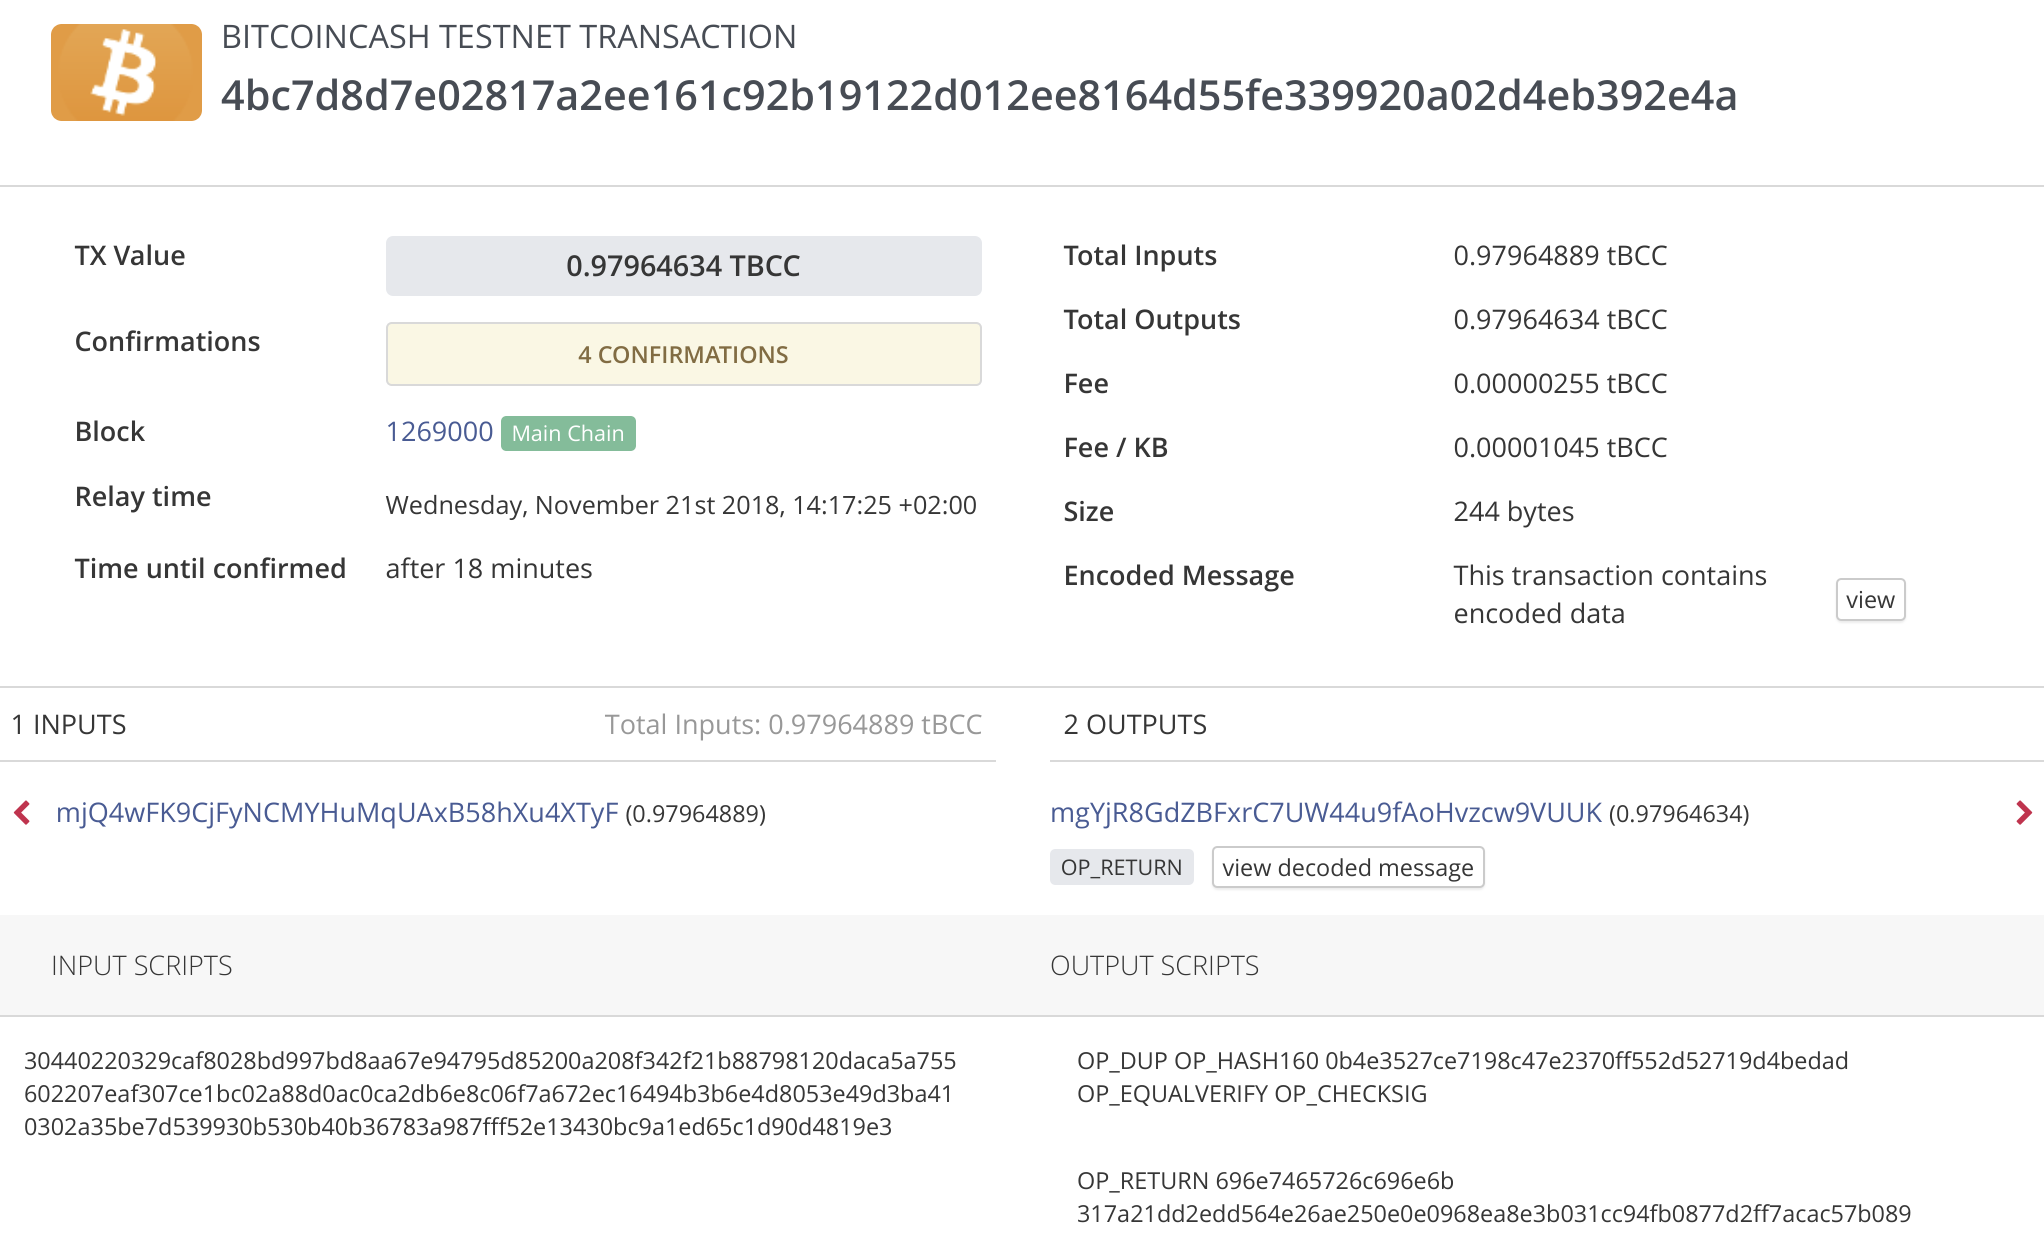
\includegraphics[width=0.9\columnwidth,keepaspectratio]{figures/actual-velvet-tx.png}
  \caption{An actual velvet fork transaction.}
  \label{fig:actual-velvet-tx}
\end{figure}

\section{Fault Tolerance}
It is important to note that the interlinker works on a best-effort basis. Due to the nature of Velvet Forks though, no failure is fatal. The types of failures are as follows:

\begin{itemize}
  \item \textbf{Crash failure}: The interlinker crashes or halts.
  \item \textbf{Omission failure}: The interlinker fails to push a transaction upon seeing a new block.
  \item \textbf{Timing failure}: The interlinker pushes a transaction which fails to be included in the upcoming block.
  \item \textbf{Response failure}: The interlinker pushes a transaction with an invalid interlink.
  \item \textbf{Arbitrary failure}: The interlinker pushes a transaction before a new block is seen or pushes a duplicate for a specific upcoming block twice.
\end{itemize}

We will study how these failures can be mitigated in the next section.

\section{Viability}
Making the operation of the interlinker affordable is key in order to allow many parties to run it. We will estimate the cost of operation now.

Our transaction size ($\sf txBytes$) is constant at exactly 244 bytes. The median Bitcoin Cash fee per byte ($\sf feePerByte$) at the time of writing (November 2018) is 1 satoshi. Multiplied by our transaction size this gives us a transaction fee ($\sf txFee = txBytes * feePerByte$) of 244 satoshis.

\begin{table}
  \centering
  \begin{tabular}{|c|c|c|}
    \hline
    Cost per & Formula & Current estimation \\
    \hline
    Day & $\sf txFee * 10 * 24$ & 0.13€ \\
    Month & $\sf perDay * 30$ & 3.9€ \\
    Year & $\sf perMonth * 12$ & 46.8€ \\
    \hline
  \end{tabular}
\end{table}

We provide two implementations of an interlinker which both run in production. We'll now look at the pros and cons of each.

\section{Bitcoin-ABC}
Our first implementation is built on top of Bitcoin-ABC. Bitcoin-ABC is the reference implementation for Bitcoin Cash in C++. It is a fork of the original Bitcoin codebase (now Bitcoin Core), and it was the first ever implementation to support Bitcoin Cash. It has a very active community of developers and users. Due to its heritage from Bitcoin Core the code is very well written and tested, and any new feature for the Bitcoin Cash chain appears on Bitcoin-ABC first.

We run Bitcoin-ABC as a full node and interface with it using JSON-RPC. The interlinker is a Python module which knows (a) the location and credentials to connect with the full node and (b) the velvet fork genesis block id.

After the interlinker makes sure the full node is fully synced it starts waiting for new blocks. As described above we need our interlinker to get notified whenever there's a new block so that it can send a transaction with the new interlink for inclusion in the upcoming block. There's two options to get notified for new blocks from a full node.

The first option is to utilize the ZeroMQ~\cite{zmq} functionality of Bitcoin-ABC. If compiled with the appropriate flags, Bitcoin-ABC can create a ZeroMQ channel where it will send notifications for new blocks and transactions. While the method seems very modern, it has some pitfalls. The main pitfall is race conditions: it is possible that the node pushes out a ZeroMQ notification about a block, however that block has not finished saving in the node's database, causing an immediate \code{getblock} request on the block to fail. Also, the ZeroMQ functionality is not enabled by default: one needs to compile the node with specific flags. While both issues are not fatal, in order to keep the interlinker as compatible with existing nodes as possible and to avoid workarounds we decided against using this functionality.

What we ended up using is busy polling through JSON-RPC with the \code{getbestblockhash} method. Every 5 seconds the interlinker will check the best block hash and if it doesn't match the one previously given then this means that there's been a new block. The interval can be configured should one desire not to cause much strain to their system.

In case there's a new block, the interlinker will promptly compute the correct interlink for it, by updating the interlink with all the intermediate blocks from the velvet fork genesis up to and including the new block. It will then compute the Merkle Tree root and include it in an SPV tagged output. It will then wrap the output inside a change transaction and send it to the network.

It is important to note here that in order to send the transactions, the interlinker has to pay transaction fees as seen earlier. However, we haven't talked about the interlinker controlling a wallet or private keys which would make it seem like there is no way to fund the transactions. Because of how the JSON-RPC methods work we don't need to specify a private key or wallet external to the full node and we can let the full node create and pay for our transactions using its default wallet. Thus the way to fund the interlinker is to fund the default wallet of the full node.

code snippets TODO

\section{bcash}
The second implementation is build on top of the bcash JavaScript library. bcash implements a full node and wallet functionality exclusively in JavaScript without being based on the Bitcoin C++ codebase as did most previous solutions. A major advantage of bcash is that it implements an SPV node too, which is very useful since the interlinker only needs the block ids of the chain but doesn't care about the block contents, so requiring a full node to run it would be a waste of space and bandwidth.

\section{Deployment}
At the time of writing of this thesis, both interlinkers run in production on the Bitcoin Cash testnet chain and have been for over 2 months. We started with our first deployment late September 2018, with the first prototype of our Python interlinker. This gave us a chance to catch bugs that only appear on long running processes and make sure our software is resilient to network and other library failures. As new features and bug fixes kept rolling in our software we continuously updated the deployments.

docker images
docker-compose

\section{Experimental Data}
\begin{figure}
  \centering
  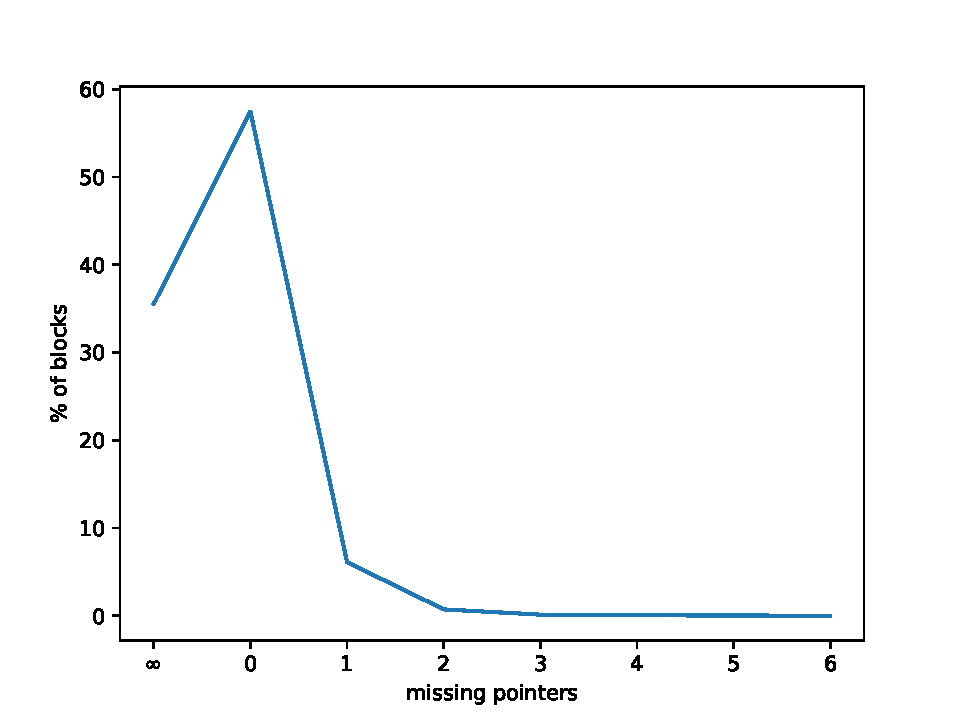
\includegraphics[width=0.9\columnwidth,keepaspectratio]{figures/testnet-deployment-reliability.pdf}
  \caption{Reliability of our testnet deployment.}
  \label{fig:testnet-deployment-reliability}
\end{figure}

We will now examine real-world data gathered from our Bitcoin Cash testnet deployment. On Figure~\ref{fig:testnet-deployment-reliability} we can look at the reliability of our interlinker deployment. We can see that about 60\% of the blocks have been correctly interlinked with our velvet transactions, and about 10\% of them only have 1 interlink pointer missing, which makes them potentially usable. With $\infty$ we denote the case where all pointers are missing due to a block only having incorrect interlinks or no interlinks at all.

\begin{figure}
  \centering
  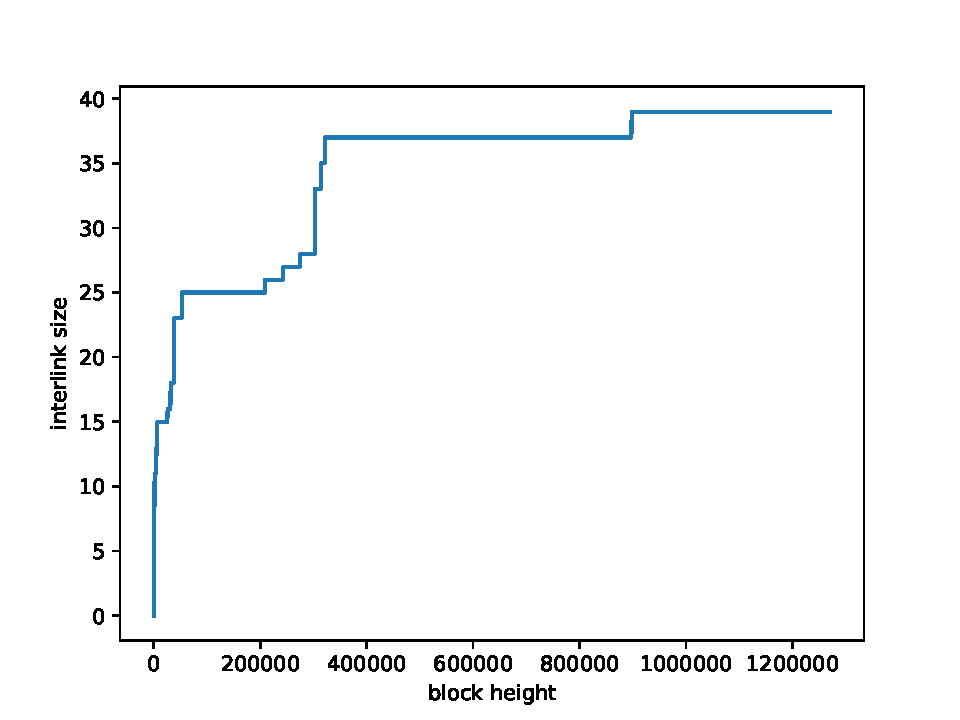
\includegraphics[width=0.9\columnwidth,keepaspectratio]{figures/bitcoin-cash-testnet-levels.pdf}
  \caption{Level distribution on Bitcoin Cash testnet.}
  \label{fig:bitcoin-cash-testnet-levels}
\end{figure}

On Figure~\ref{fig:bitcoin-cash-testnet-levels} we see the level distribution on the Bitcoin Cash testnet. As expected, the level growth is logarithmic compared to the chain length.

\chapter{NIPoPoW Velvet Fork Prover}
Now that we've established a fork on the Bitcoin Cash chain, we show how our fork can be put to use by creating proofs. We introduce a kind of client called a \emph{prover} which can create all kinds of NIPoPoW proofs on demand.

Let's assume we have an SPV node. We set the bloom filter to our velvet fork tag in order to get all blocks containing only the transactions of the fork. It's possible to then extract from each transaction the payload, which should be the interlink commitment. Since anyone can post such transactions on the blockchain, we have to make sure that the commitment is actually true before we can use it. In order to do that we maintain our own version of the interlink for each block (similar to how the interlinker does) which we know is correct called $\sf realLink$. Then for every block, we compare its commitments (there may be many) with the Merkle Tree root of our $\sf realLink$. If there is a valid commitment we say that the block has a valid interlink. We store the full interlink as $\sf realLink[id(block)]$.

When we talked about NIPoPoWs we mentioned how it's essential that our proof forms a blockchain that can be traversed from start to end. In order to make our proof traversable, whenever we include a block we have to make sure it connects validly to the previous one either by (a) using the regular $\sf previd$ inside the block or (b) using a valid interlink. If we use the $\sf previd$ to link back to the previous block then all the information someone needs to verify the traversability is already there and we don't need to add anything extra. In the case we use the interlink however, we need to provide the Merkle Tree proofs for:

\begin{itemize}
  \item The transaction containing the valid interlink commitment.
  \item The interlink level we use for the connection.
\end{itemize}

If our chain is not traversable the proof is automatically invalid.

We'll now look at the concrete implementation of the prover.

\section{Invalid Interlink Handling}
The original NIPoPoWs paper~\cite{nipopows} gives us some insight into how to handle blocks with invalid interlinks. Let's look at where we need to make changes starting with suffix proofs.

For suffix proofs we need a way to obtain the upchain of a chain, denoted as $\chain\upchain^\mu$. We will now define a procedure to programatically obtain the upchain of a chain called $\sf find \chain\upchain^\mu$.

\subsection{\sf followUp}
$\sf followUp$ takes a block $b$ and a level $\mu$ as parameters. Starting from $b$ it traverses the chain until it reaches another block of level $\mu$ called $B$. In doing so, it is only allowed to use valid pointers. It will only follow a pointer from a block's interlink at level $\mu$ if there is a valid interlink in that block. Otherwise, the only option is to follow the previous block pointer ($\sf previd$). Once $B$ is reached, it is returned alongside the blocks that were traversed as a blockset called $\sf aux$.

\begin{algorithm}[H]
    \caption{\label{alg.nipopow-velvet-follow}followUp
    produces the blocks to connect two superblocks in velvet forks.}
    \begin{algorithmic}[1]
        \Function{\sf followUp}{$B$, $\mu$, realLink, blockById}
            \Let{\textsf{aux}}{\{B\}}
            \While{$B \neq \textsf{Gen}$}
                \If{$B.\textsf{interlink}[\mu] = \textsf{realLink}[\textsf{id}(B)][\mu]$}
                    \Let{id}{B.\textsf{interlink}[\mu]}
                \Else
                    \Comment{Invalid interlink}
                    \Let{id}{B.\textsf{previd}}
                \EndIf
                \Let{B}{\textsf{blockById}[id]}
                \Let{\textsf{aux}}{\textsf{aux}\cup \{B\}}
                \If{$\textit{level}(B) = \mu$}
                    \State\Return{$B$, aux}
                \EndIf
            \EndWhile
            \State\Return{$B$, aux}
        \EndFunction
    \vskip8pt
    \end{algorithmic}
\end{algorithm}


%TODO figure with straight and dropdown cases

\subsection{$\sf find \chain\upchain^\mu$}
Now that we have a way to go back on a level, we can utilize it to construct the entire traversable level $\mu$ up to block $b$, starting from the end of the chain $\chain[-1]$: this is what ${\sf find \chain\upchain^\mu}(b)$ accomplishes. It works by repeatedly calling $\sf followUp$ on the oldest block it has and including the result in its final chain.

\begin{algorithm}[H]
    \caption{\label{alg.nipopow-velvet-upchain}Supplying the necessary data
    to calculate a connected $\chain\upchain^\mu$ during a velvet fork.}
    \begin{algorithmic}[1]
        \Function{{\sf find} $\chain\upchain^\mu$}{$b$, realLink, blockById}
            \Let{B}{\chain[-1]}
            \Let{\textsf{aux}}{\{B\}}
            \Let{\pi}{[~]}
            \If{$\textit{level}(B) \geq \mu$}
                \Let{\pi}{\pi B}
            \EndIf
            \While{$B \neq b$}
                \State $(B, \textsf{aux'})$
                \begin{varwidth}[t]{\linewidth}
                    $\gets$
                    \textsf{followUp}$(B, \mu,
                    \textsf{realLink}, \textsf{blockById})$
                \end{varwidth}
                \Let{\textsf{aux}}{\textsf{aux} \cup \textsf{aux'}}
                \Let{\pi}{\pi B}
            \EndWhile
            \State\Return{$\pi$, aux}
        \EndFunction
    \vskip8pt
    \end{algorithmic}
\end{algorithm}


\section{Velvet Infix Proofs}

\begin{algorithm}[H]
    \caption{\label{alg.nipopow-velvet-infix-go-back}The \textsf{goBack} function which produces the necessary blocks to connect a block $right$ to a preceeding block $left$.}
    \begin{algorithmic}[1]
        \Function{\sf goBack}{$left$, $right$, \textsf{height}, \textsf{realLink}, \textsf{blockById}}
            \State{$aux \gets \emptyset$}
            \While{$right \neq left$}
                \For{$\mu = level(left)$ down to $0$}
                    \If{$\textsf{realLink}[\mathsf{id}(right)][\mu] = right\text{.interlink}[\mu]$}
                        \Let{B'}{\textsf{blockById}[right\text{.interlink}[\mu]]}
                        \If{$\textsf{height}[B'] \ge \textsf{height}[left]$}
                            \Let{aux}{aux \cup \{B'\}}
                            \Let{right}{B'}
                            \State\textbf{break}
                        \EndIf
                    \EndIf
                \EndFor
            \EndWhile
            \State\Return{$aux$}
        \EndFunction
    \vskip8pt
    \end{algorithmic}
\end{algorithm}


\section{JavaScript implementation with bcash}
bcash, also used for the interlinker earlier, turns out the be the only option for an SPV node on Bitcoin Cash, making it the obvious choice for the prover.

\subsection{Overview}
Our prover works as follows. We expect a user to run the prover, passing as a parameter if they want a suffix or infix proof. If they desire an infix proof they have to provide the block of interest. Once they do that the prover runs and syncs with the Bitcoin Cash blockchain via SPV. It does some similar work to the work that an interlinker does: it knows what the correct interlink is for each block. It then checks the included commitments on each block and keeps a valid commitment for each block if found. A block containing a valid commitment is called a \emph{valid velvet}. Interlink pointers can only be used on valid velvets. Once the chain is synced and the prover knows the valid velvets along with the whole blockchain it creates a proof of the requested type and outputs it in JSON format.

\subsection{Interlink Implementation}
Implementing an interlink structure is something we've already covered many times. Our implementation here is based on immutable value objects holding the interlink. Updating an interlink is done in the usual manner and creates a new interlink. What's different here is that we have a \code{proof} method: we use this method to generate a proof of inclusion of a specific pointer in the interlink commitment. We also need a way to be able to get a pointer from a specific level on the interlink and this is accomplished with the \code{at} method. Note that \code{at} can be asked for a level higher than the size of the interlink, in which case the velvet genesis is returned as it's assumed to be a block of level $\infty$.

\begin{lstlisting}[language=Javascript]
class Interlink {
  list: Array<BlockId>;
  genesisId: BlockId;

  constructor(genesisId: BlockId, list: Array<BlockId> = []) {
    this.genesisId = genesisId;
    this.list = list;
  }

  update(blockId: BlockId) {
    const list = this.list.slice();
    const lvl = level(blockId);
    for (let i = 0; i <= lvl; ++i) {
      if (i < list.length) list[i] = blockId;
      else list.push(blockId);
    }
    return new Interlink(this.genesisId, list);
  }

  proof(level: number) {
    return merkle.createBranch(hash256, level, [...this.list]);
  }

  hash() {
    return merkle.createRoot(hash256, [...this.list])[0];
  }

  get length() {
    return this.list.length;
  }

  at(lvl: number) {
    if (lvl >= this.list.length) {
      return this.genesisId;
    }
    return this.list[lvl];
  }
}
\end{lstlisting}

\subsection{Locating Velvet Transactions}
Locating the velvet transactions is very easy considering that all our velvet transactions are SPV tagged. The only thing we have to do is add the SPV tag in our bloom filter. We do this right before connecting to the network.

\begin{lstlisting}[language=Javascript]
module.exports = class ProverNode extends bcash.SPVNode {
  // ...
  async connect() {
    this.pool.watch(Buffer.from(VELVET_FORK_MARKER));
    await super.connect();
  }
  // ...
}
\end{lstlisting}

\subsection{Extracting Interlink Commitments}
we have to check that the transaction the valid form described earlier (\code{OP\_RETURN <tag> <commitment>}). In order to do that we look at the outputs of each transaction and only keep any outputs of our form. If some output matches then we extract the script's third element which is the commitment.

\begin{lstlisting}[language=Javascript]
const extractInterlinkHashes = compose(
  map(
    compose(
      head,
      drop(1)
    )
  ),
  filter(isInterlinkData),
  map(
    compose(
      getCleanScriptData,
      prop("script")
    )
  ),
  filter(isBurnOutput),
  prop("outputs")
);
\end{lstlisting}

\subsection{Handling Merkle Blocks}
When a block or transaction of a block matches our bloom filter, the block is relayed by full nodes as a \code{merkleblock} message. MerkleBlocks contain the header of the actual block as well as the transactions ids that matched. It also contains a proof of inclusion for all the transactions ids provided. One can check this proof of inclusion with accordance to the \code{merkleRoot} inside the block header. The transactions are included in subsequent \code{tx} messages. bcash hides this process from the user: on a new block event a MerkleBlock is provided and it contains a \code{txs} record, where the transactions that matched are included in full.

In order to check if we have matched transactions in a block all we have to do is check if its \code{.txs} array is non-empty. If it is not then this block is definitely not a valid velvet. If it is not, then we have to ensure a correct form and extract the commitment, also saving it. We utilize the method \code{extractInterlinkHashes} and map it over all transactions in the block.

\begin{lstlisting}[language=Javascript]
const extractInterlinkHashesFromMerkleBlock = compose(
  unnest,
  map(extractInterlinkHashes),
  prop("txs")
);
\end{lstlisting}

\subsection{RealLink \& Verifying Interlink Commitments}
We extend the \code{realLink} discussed earlier. Other than allowing us to get the interlink of any block it also allows us to check if a block is a valid velvet. It is able to do that as it gets notified for every new block seen during the synchronisation. When a new block appears, it gets informed about the block id and the interlinks included in the block. It keeps a running interlink in the same fashion the interlinker does so because the blocks events happen in-order it can check whether its running interlink matches the ones included in the block. In case there's a match the block is marked as a valid velvet and the running interlink is updated so that RealLink can be ready to process the next block.

\begin{lstlisting}[language=Javascript]
module.exports = class RealLink {
  blockIdToInterlink: BufferMap;
  runningInterlink: Interlink;
  validBlocks: BufferSet;

  constructor(genesisId: BlockId) {
    this.blockIdToInterlink = new BufferMap();
    this.runningInterlink = new Interlink(genesisId);
    this.validBlocks = new BufferSet();
  }

  onBlock(newBlockId: BlockId, interlinks: Array<Buffer>) {
    if (this.blockIdToInterlink.has(newBlockId)) {
      return;
    }

    this.blockIdToInterlink.set(newBlockId, this.runningInterlink);
    if (
      interlinks.some(interlink =>
        interlink.equals(this.runningInterlink.hash())
      )
    ) {
      this.validBlocks.add(newBlockId);
    }
    this.runningInterlink = this.runningInterlink.update(newBlockId);
  }

  get(blockId: BlockId) {
    return this.blockIdToInterlink.get(blockId);
  }

  hasValidInterlink(blockId: BlockId) {
    return this.validBlocks.has(blockId);
  }
};
\end{lstlisting}

\subsection{Handling Merkle Blocks Redux}
All information regarding the chain is sorted in a \code{VelvetChain} (TODO change name). A \code{VelvetChain} is the main entrypoint for block events. It is the single source of truth about the blockchain. When there is a new block, the whole block is associated with its id for later lookup, and its height is also recorded. It then gathers the block's interlink commitments and forwards them as a new event to \code{realLink}.

\begin{lstlisting}[language=Javascript]
  // ...
  onBlock(blk: bcash.MerkleBlock, height: number) {
    const id = blk.hash();
    if (this.blockById.has(id)) {
      return;
    }

    ++this.height;

    if (!this.genesis) {
      this.genesis = id;
      this._realLink = new RealLink(this.genesis);
      console.log("genesis was %O", blk);
    }

    this.blockById.set(id, blk);
    this.heightById.set(id, this.height);
    this.blockList.push(blk.hash());

    const includedInterlinkHashes = extractInterlinkHashesFromMerkleBlock(blk);
    this.realLink.onBlock(id, includedInterlinkHashes);

    this.lastBlock = id;
  }
  // ...
\end{lstlisting}

\subsection{Following Up}
\subsection{Finding the Velvet Upchain}
\subsection{Crafting Suffix Proofs}
\subsection{Following Down}
\subsection{Going Back}
\subsection{Crafting Infix Proofs}

\subsection{Type Safety}
To ensure code quality we opted to use Flow~\cite{flow}. Flow allowed us to have type safety while keeping all the good characteristics of JavaScript. Unfortunately this introduced a couple of complications.

One is that our source files are not valid JavaScript anymore. In order to run our code we need to pass it through a pre-processor like Babel which emits clean JavaScript that then Node can run.

Another is that all the external libraries we use, including bcash are not written including Flow types. Flow does provide a repository with type definitions for popular packages, however due to the niche category of our dependencies only a few were covered. This meant that the burden was on us to write type definitions for our dependencies. We had to manually write type definitions for bcash and buffer-map. Thankfully, there is previous work~\footnote{Available at \url{https://github.com/OrfeasLitos/TrustIsRisk.js/blob/247c8b182f5bb4bed11df0d3b9136a3e27848798/flow-typed/npm/bcoin_vx.x.x.js}} on type definitions for bcoin which we were able to utilize and extend since the APIs are really similar as bcash is a fork of bcoin.

\subsection{Testing}
Due to the real-time and asynchronous nature of the prover it's important that our implementation is resilient and bug-free. In order to assert that the code has been thoroughly unit tested, boasting a code coverage of >90\%. The tests are written and run with Jest~\cite{jest}. There are also integration tests using real-world data.

\chapter{Conclusion}

\section{Summary}
\section{Proof Consumption}
\section{Future Work}


\bibliography{bibliography}

\end{document}
